\documentclass[crop,tikz]{standalone}
\usetikzlibrary{arrows.meta}
\begin{document}
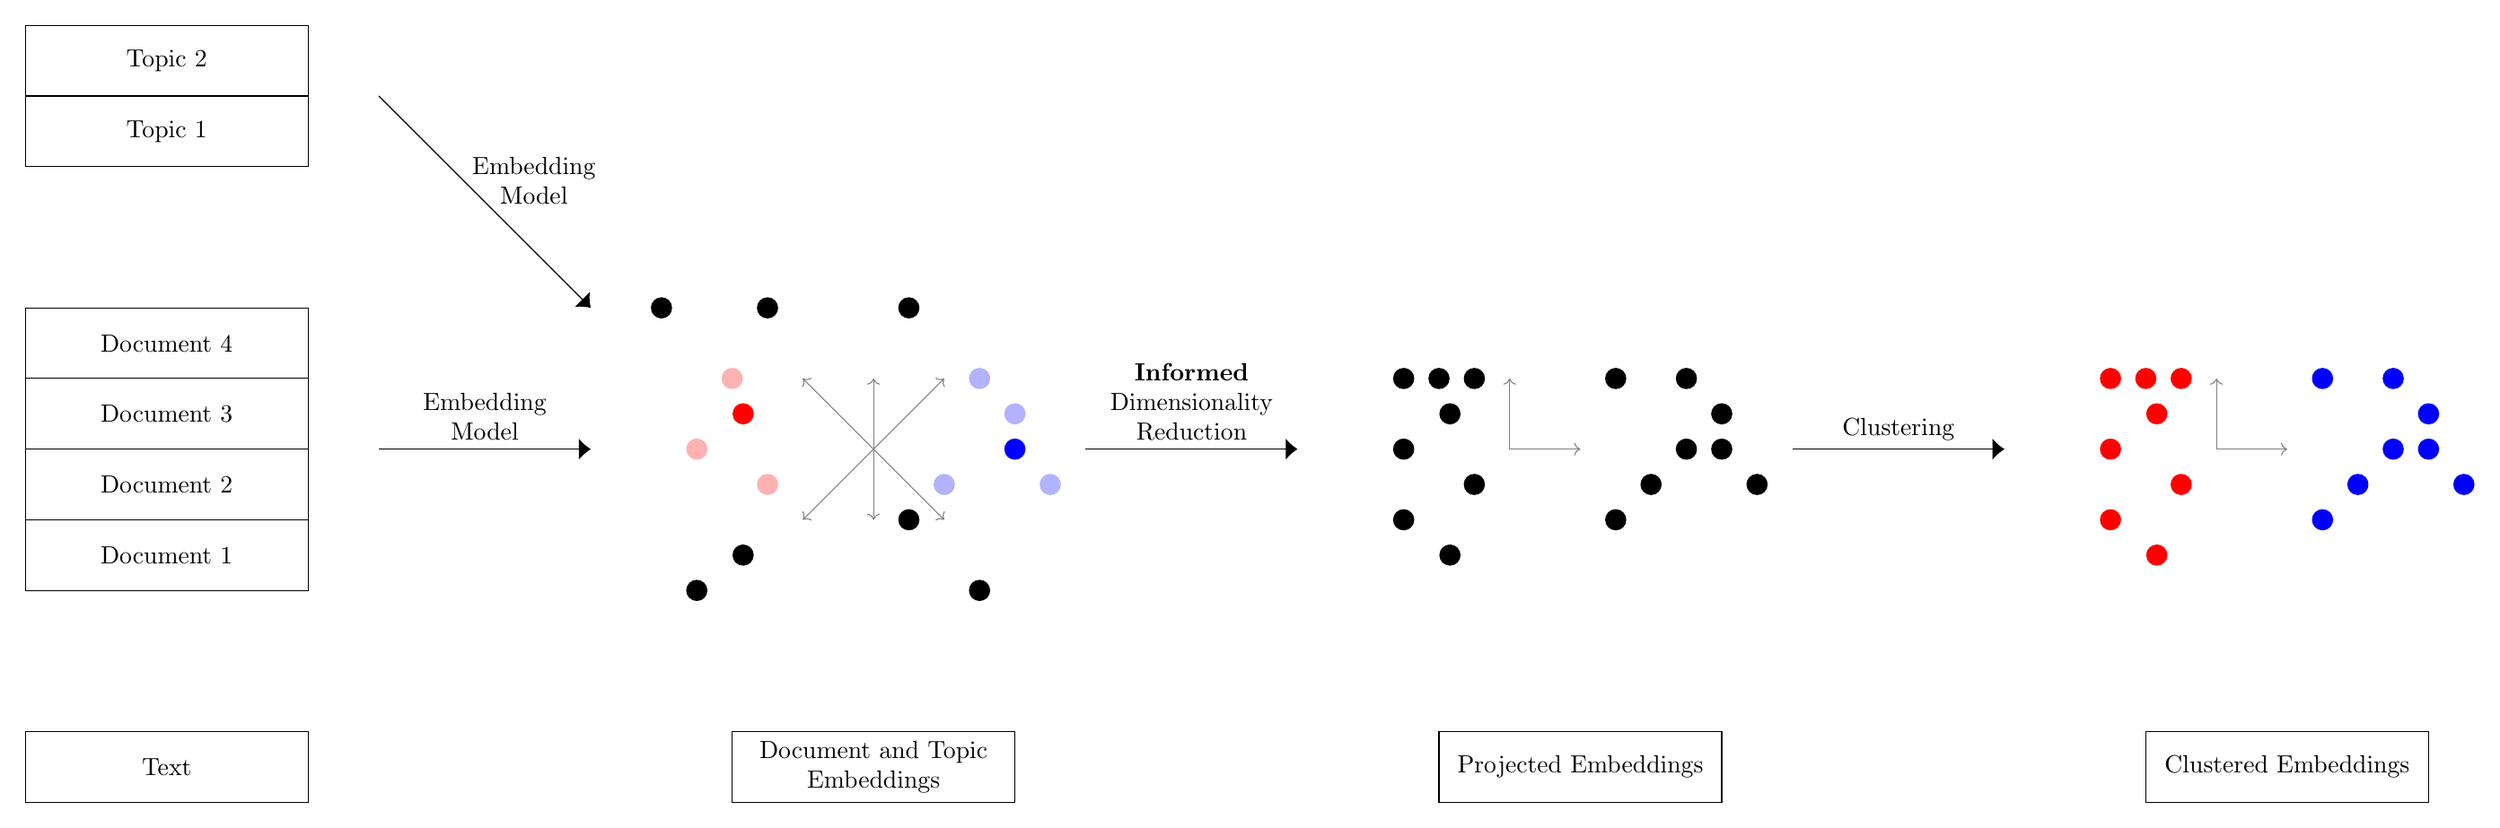
\begin{tikzpicture}

  \draw (0, -2) rectangle (4,-1) node[pos=.5] {Text};

  \draw (0,1) rectangle (4,2) node[pos=.5] {Document 1};
  \draw (0,2) rectangle (4,3) node[pos=.5] {Document 2};
  \draw (0,3) rectangle (4,4) node[pos=.5] {Document 3};
  \draw (0,4) rectangle (4,5) node[pos=.5] {Document 4};

  \draw (0,7) rectangle (4,8) node[pos=.5] {Topic 1};
  \draw (0,8) rectangle (4,9) node[pos=.5] {Topic 2};

  \draw (10, -2) rectangle (14,-1) node[pos=.5, align=center] {Document and Topic\\Embeddings};

  \draw[->, gray] (12, 3) -- (12, 4);
  \draw[->, gray] (12, 3) -- (13, 4);
  \draw[->, gray] (12, 3) -- (11, 4);
  \draw[->, gray] (12, 3) -- (11, 2);
  \draw[->, gray] (12, 3) -- (13, 2);
  \draw[->, gray] (12, 3) -- (12, 2);

  \fill[red!30] (2+8, 4) circle (.15) node {};
  \fill (2+8.5, 5) circle (.15) node {};
  \fill (2+7, 5) circle (.15) node {};
  \fill[red!30] (2+7.5, 3) circle (.15) node {};
  \fill[red] (2+8.155, 3.5) circle (.15) node {};
  \fill[red!30] (2+8.5, 2.5) circle (.15) node {};
  \fill (2+7.5, 1) circle (.15) node {};
  \fill (2+8.155, 1.5) circle (.15) node {};

  \fill[blue!30] (6+7, 2.5) circle (.15) node {};
  \fill (6+6.5, 5) circle (.15) node {};
  \fill[blue!30] (6+7.5, 4) circle (.15) node {};
  \fill[blue] (6+8, 3) circle (.15) node {};
  \fill[blue!30] (6+8, 3.5) circle (.15) node {};
  \fill[blue!30] (6+8.5, 2.5) circle (.15) node {};
  \fill (6+6.5, 2) circle (.15) node {};
  \fill (6+7.5, 1) circle (.15) node {};

  \draw (20, -2) rectangle (24,-1) node[pos=.5] {Projected Embeddings};
  \draw[->, gray] (21, 3) -- (21, 4);
  \draw[->, gray] (21, 3) -- (22, 3);

  \fill (12+8, 4) circle (.15) node {};
  \fill (12+8.5, 4) circle (.15) node {};
  \fill (12+7.5, 4) circle (.15) node {};
  \fill (12+7.5, 3) circle (.15) node {};
  \fill (12+8.155, 3.5) circle (.15) node {};
  \fill (12+8.5, 2.5) circle (.15) node {};
  \fill (12+7.5, 2) circle (.15) node {};
  \fill (12+8.155, 1.5) circle (.15) node {};

  \fill (16+7, 2.5) circle (.15) node {};
  \fill (16+6.5, 4) circle (.15) node {};
  \fill (16+7.5, 4) circle (.15) node {};
  \fill (16+8, 3) circle (.15) node {};
  \fill (16+8, 3.5) circle (.15) node {};
  \fill (16+8.5, 2.5) circle (.15) node {};
  \fill (16+6.5, 2) circle (.15) node {};
  \fill (16+7.5, 3) circle (.15) node {};

  \draw (30, -2) rectangle (34,-1) node[pos=.5] {Clustered Embeddings};
  \draw[->, gray] (31, 3) -- (31, 4);
  \draw[->, gray] (31, 3) -- (32, 3);

  \fill[red] (22+8, 4) circle (.15) node {};
  \fill[red] (22+8.5, 4) circle (.15) node {};
  \fill[red] (22+7.5, 4) circle (.15) node {};
  \fill[red] (22+7.5, 3) circle (.15) node {};
  \fill[red] (22+8.155, 3.5) circle (.15) node {};
  \fill[red] (22+8.5, 2.5) circle (.15) node {};
  \fill[red] (22+7.5, 2) circle (.15) node {};
  \fill[red] (22+8.155, 1.5) circle (.15) node {};

  \fill[blue] (26+7, 2.5) circle (.15) node {};
  \fill[blue] (26+6.5, 4) circle (.15) node {};
  \fill[blue] (26+7.5, 4) circle (.15) node {};
  \fill[blue] (26+8, 3) circle (.15) node {};
  \fill[blue] (26+8, 3.5) circle (.15) node {};
  \fill[blue] (26+8.5, 2.5) circle (.15) node {};
  \fill[blue] (26+6.5, 2) circle (.15) node {};
  \fill[blue] (26+7.5, 3) circle (.15) node {};

  \draw[-{Latex[width=3mm]}] (5, 3) -- (8, 3) node[pos=.5, anchor=south, align=center] {Embedding\\Model};
  \draw[-{Latex[width=3mm]}] (5, 8) -- (8, 5) node[pos=.4, anchor=west, align=center] {Embedding\\Model};

  \draw[-{Latex[width=3mm]}] (15, 3) -- (18, 3) node[pos=.5, anchor=south, align=center] {\textbf{Informed}\\Dimensionality\\Reduction};
  \draw[-{Latex[width=3mm]}] (25, 3) -- (28, 3) node[pos=.5, anchor=south] {Clustering};

\end{tikzpicture}
\end{document}